\chapter{Methodology}
\label{chapter:methodology}

\section{Architecture Overview}
\label{section:architecture_overview}

In this dissertation, I propose a . The proposed model comprises four main components, as outlined below. A high-level overview of the model is shown in \figureautorefname{ \ref{TODO}}

\begin{itemize}
  \item Question input module
  \item Scene graph input module (knowledge base)
  \item Reasoning module
  \item Output module
\end{itemize}

\begin{figure}[htbp]
    \centering
    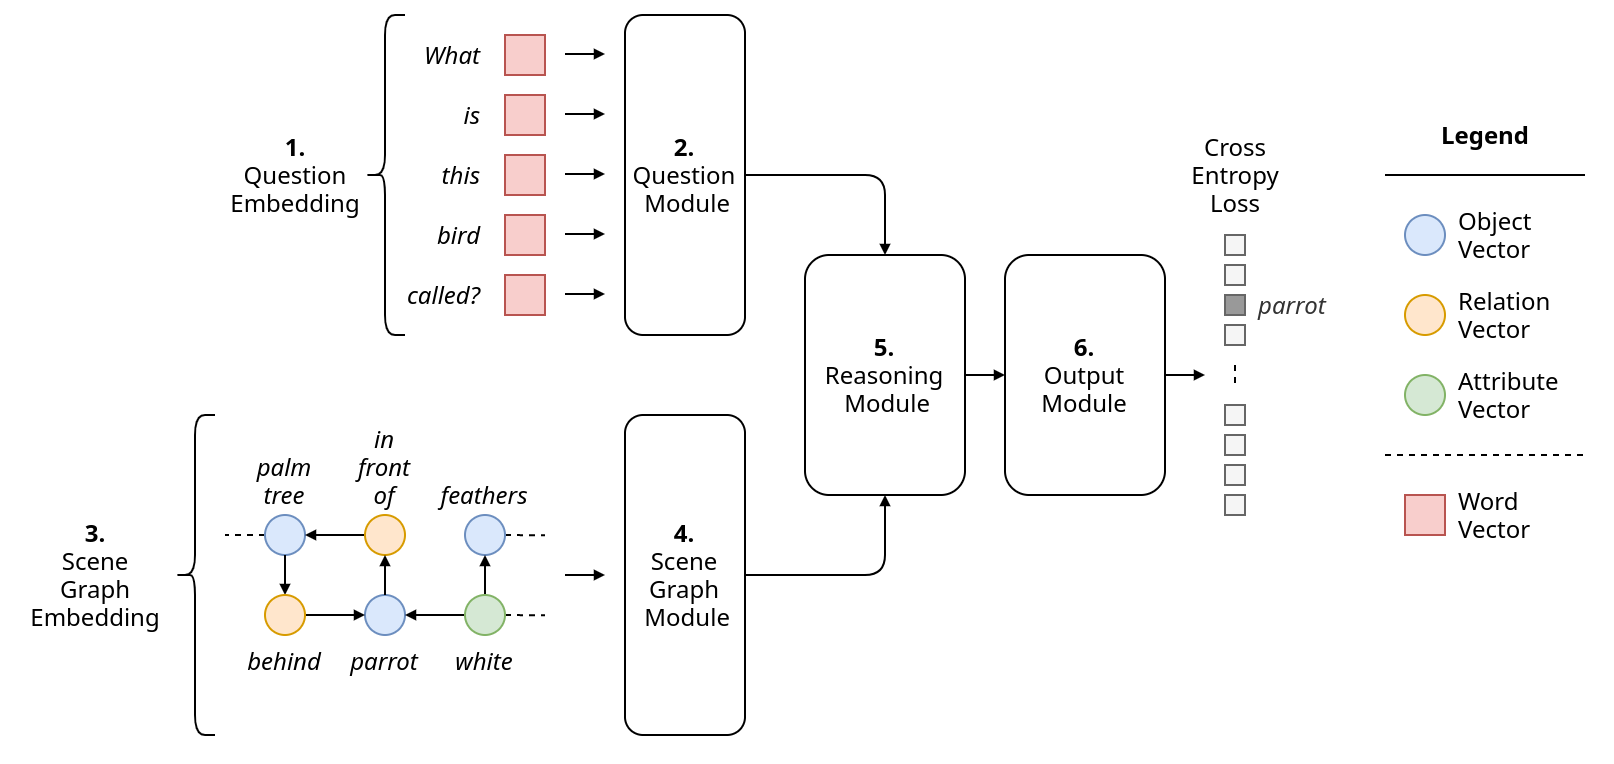
\includegraphics[width=\textwidth]{model.png}
    \caption{A high-level overview of the proposed visual-question-answering model.}
    \label{fig:model_overview}
\end{figure}

\section{Question Input Module}
\label{section:question_input_module}

\section{Scene Graph Input Module}
\label{section:scene_graph_input_module}

\section{Compositional Attention Network}
\label{section:compositional_attention_network}

{\color{red}

Move to Ablations

\begin{itemize}
  \item Concat + linear fusion (other fusion types?)
  \item Bottom-up
  \item MAC network
\end{itemize}

\subsection{Bottom-up}
\label{subsection:bottom_up}
 ReLU proved to yield higher results over gated tanh when paired with GAT/GCN embeddings. In the original paper, CNN/R-CNN features are extracted in the preprocessing step, meaning there is no need for gradient propagation to the knowledge base embedding. Preliminary tests showed a need for learnable embeddings in graph convolutional models, and thus a need for end-to-end propagation of gradients.}


In order to leverage the computational benefits of sparse tensor operations implemented in PyG \cite{fey2019fast}, I used a PyTorch \cite{paszke2019pytorch} re-implementation of the MAC network, which has been trained to 98.6\% on the CLEVR dataset \cite{eyzaguirre2020differentiable}, just 0.3\% shy of the official result reported by 
\citeauthor{hudson2018compositional}. Notably, this re-implementation accounts for minor details that were omitted from the original MAC network paper but enabled by default in the official MAC network repository {\color{red} citation required}.

\begin{itemize}
  \item Initial tests showed little performance difference between conditioning the current control state on previous control states. % #TODOInvestigate interpretability effects
\end{itemize}
